\documentclass{beamer}
%\documentclass[handout,t]{beamer}

\batchmode
% \usepackage{pgfpages}
% \pgfpagesuselayout{4 on 1}[letterpaper,landscape,border shrink=5mm]

\usepackage{amsmath,amssymb,enumerate,epsfig,bbm,calc,color,ifthen,capt-of}

% TikZ packages
\usepackage{tikz}
\usetikzlibrary{arrows,decorations.pathmorphing,decorations.footprints,fadings,calc,trees,mindmap,shadows,decorations.text,patterns,positioning,shapes,matrix,fit}


\usetheme{Berlin}
\usecolortheme{mit}

\title{The OpenMC Monte Carlo Code}
\author{Paul K. Romano}
\date{October 6, 2011}
\pgfdeclareimage[height=0.5cm]{mit-logo}{mit-logo.pdf}
\logo{\pgfuseimage{mit-logo}\hspace*{0.3cm}}

\AtBeginSection[]
{
  \begin{frame}<beamer>
    \frametitle{Outline}
    \tableofcontents[currentsection]
  \end{frame}
}
\beamerdefaultoverlayspecification{<+->}

\tikzstyle{sNormalBlockStyle} =
[
	draw,
	rectangle,
	rounded corners	= 0.1cm,
	fill			= blue!20,
	minimum height	= 3em,
	minimum width   = 6em,
]

\tikzstyle{RectBlue} =
[
	draw,
	rectangle,
	fill			= blue!20,
	minimum height	= 2em,
	minimum width	= 2em,
]

\tikzstyle{RectGreen} =
[
	draw,
	rectangle,
	fill			= green!20,
	minimum height	= 2em,
	minimum width	= 2em,
]

\tikzstyle{RectWhite} =
[
	draw,
	rectangle,
	minimum height	= 2em,
	minimum width	= 2em,
]

\tikzstyle{sTextBlockStyle} =
[
	draw,
	rectangle,
	drop shadow,
	rounded corners	= 0.1cm,
	fill			= blue!10,
	thick,
	inner xsep		= 0.2cm,		% minimum distance between text and borders along x dimension
	inner ysep		= 0.2cm 		% minimum distance between text and borders along y dimension
]


% -----------------------------------------------------------------------------
\begin{document}
% -----------------------------------------------------------------------------

\frame{\titlepage}

\section[Outline]{}
\begin{frame}{Outline}
  \tableofcontents
\end{frame}

% -----------------------------------------------------------------------------
\section{Introduction}

\begin{frame}{Background}
  My background:
  \begin{itemize}
    \item<1-> B.S. Nuclear Engineering, RPI (2007)
    \item<1-> M.S. Nuclear Scince and Engineering, MIT (2009)
  \end{itemize}
  Origin of OpenMC:
  \begin{itemize}
    \item<1-> Working on advanced parallelization for Monte Carlo
    \item<1-> Needed testing platform - MC21?
    \item<1-> Ultimately decided to start from scratch
  \end{itemize}
\end{frame}

\begin{frame}{Goals}
  Overall objectives of OpenMC:
  \begin{itemize}
  \item<1-> Fully featured, capable of realistic physics
  \item<1-> Written in a modern programming language (F2003)
  \item<1-> Easy to understand inner workings
  \item<1-> High performance
  \item<1-> Extensible for research purposes
  \item<1-> Open source and freely available
  \end{itemize}
\end{frame}

\begin{frame}{Monte Carlo}
  Rather than solving the transport equation by discretizing the spatial,
  energy, and angular variables, Monte Carlo solves the transport equation by
  following individual particles as they move stochastically through a medium.
  \begin{itemize}
  \item<1-> Standard deviation $\propto \frac{1}{\sqrt{N}}$
  \end{itemize}
\end{frame}

% -----------------------------------------------------------------------------
\section{Methods and Theory}

\begin{frame}{Solution Algorithm}
  \begin{itemize}
  \item<1-> Loop over particles
    \begin{enumerate}
    \item<1-> Sample particle from distribution
    \item<1-> Track particle to next collision
    \item<1-> Sample nuclide within material
    \item<1-> Sample reaction within nuclide
    \item<1-> Repeat from step 2 until particle dies
    \end{enumerate}
  \end{itemize}

  While particle is being tracked, keep track of collision rate, fission rate,
  etc.
  \begin{equation*}
    \phi = \frac{1}{NV} \sum\limits_{\text{all collisions} \atop \text{in cell}} \frac{w_i}{\Sigma_t (E_i)}
  \end{equation*}

\end{frame}

\begin{frame}{Geometry}
  \begin{itemize}
  \item<1-> All geometry is described as constructive solid geometry (unions and
    intersections of second-order surfaces)
  \item<1-> $Ax^2 + By^2 + Cz^2 + Dxy + Eyz + Fxz + Gx + Hy + Iz + J = 0$
  \item<1-> e.g. to construct an annulus
  \end{itemize}
  \begin{figure}
\begin{center}
\begin{tikzpicture}
[
  transform canvas = {scale=1.0},
]

\fill[mitred] (0,0) circle (1cm);
\fill[white]  (0,0) circle (0.50cm);

\end{tikzpicture}
\end{center}
\end{figure}

\end{frame}

\begin{frame}{Cross-Sections}
  \begin{itemize}
  \item<1-> No need to reinvent the wheel
  \item<1-> ACE (A Compact ENDF) Format
    \begin{itemize}
    \item<1-> MCNP
    \item<1-> SERPENT
    \end{itemize}
  \item<1-> Three arrays: NXS, JXS, XSS
  \item<1-> Parse arrays into internal derived types
  \end{itemize}
\end{frame}

\begin{frame}{Union Energy Grid}
  \begin{itemize}
  \item<1-> Each nuclide has cross-sections tabulated at different energy points
  \item<1-> To determine collision type, need to look up microscopic reaction
    cross sections
  \end{itemize}
  \begin{figure}
\begin{center}
\begin{tikzpicture}
[
  transform canvas = {scale=0.7},
  xshift = -5.0cm,
  yshift = 1.0cm
]

  \node (LabelOne)  [sTextBlockStyle]                      {Union Energy Grid};
  \node (EOne)      [RectBlue, right of = LabelOne, node distance = 3cm] {$E_1$};
  \node (ETwo)      [RectBlue, right of = EOne]   {$E_2$};
  \node (EThree)    [RectBlue, right of = ETwo]   {$E_3$};
  \node (EFour)     [RectBlue, right of = EThree] {$E_4$};
  \node (EFive)     [RectBlue, right of = EFour]  {$E_5$};
  \node (ESix)      [RectBlue, right of = EFive]  {$E_6$};
  \node (ESeven)    [RectBlue, right of = ESix]   {$E_7$};
  \node (EEight)    [RectBlue, right of = ESeven] {$E_8$};

  \node (POne)      [RectWhite, below of = EOne,   node distance = 1.5cm]   {0};
  \node (PTwo)      [RectWhite, below of = ETwo,   node distance = 1.5cm]   {0};
  \node (PThree)    [RectWhite, below of = EThree, node distance = 1.5cm]   {1};
  \node (PFour)     [RectWhite, below of = EFour,  node distance = 1.5cm]   {1};
  \node (PFive)     [RectWhite, below of = EFive,  node distance = 1.5cm]   {1};
  \node (PSix)      [RectWhite, below of = ESix,   node distance = 1.5cm]   {2};
  \node (PSeven)    [RectWhite, below of = ESeven, node distance = 1.5cm]   {3};
  \node (PEight)    [RectWhite, below of = EEight, node distance = 1.5cm]   {3};

  \node (ENucOne)   [RectGreen, below of = PThree, node distance = 1.5cm]   {$E_1$};
  \node (ENucTwo)   [RectGreen, below of = PSix,   node distance = 1.5cm]   {$E_2$};
  \node (ENucThree) [RectGreen, below of = PSeven, node distance = 1.5cm]   {$E_3$};

  \draw [-triangle 45, thick] (EOne)   -- (POne);
  \draw [-triangle 45, thick] (ETwo)   -- (PTwo);
  \draw [-triangle 45, thick] (EThree) -- (PThree);
  \draw [-triangle 45, thick] (EFour)  -- (PFour);
  \draw [-triangle 45, thick] (EFive)  -- (PFive);
  \draw [-triangle 45, thick] (ESix)   -- (PSix);
  \draw [-triangle 45, thick] (ESeven) -- (PSeven);
  \draw [-triangle 45, thick] (EEight) -- (PEight);

\end{tikzpicture}
\end{center}
\end{figure}


\end{frame}

\begin{frame}{Tallies}{}
  {\bf Remember:} In Monte Carlo, the only answer you get is the one you ask
  for. In general, you don't get the global solution like you do in
  deterministic land.
  \begin{itemize}
  \item<1-> Implemented a robust tally system to calculate user-specified
    quantities of interest
  \item<1-> {\bf Filters:} Spatial location, incoming/outgoing energy, birth region, mesh
  \item<1-> {\bf Responses:} Flux, reaction rates, currents, etc.
  \end{itemize}
\end{frame}

\begin{frame}{Parallel Fission Bank}
\end{frame}

% -----------------------------------------------------------------------------
\section{Using OpenMC}

\begin{frame}{Compiling}
\end{frame}

\begin{frame}{XML Input Format}
  Unlike many nuclear codes, OpenMC uses a modular XML input format
  \begin{itemize}
  \item<1-> Building a geometric model -- {\bf geometry.xml}
  \item<1-> Assigning materials to volumes -- {\bf materials.xml}
  \item<1-> Setting parameters for the simulation -- {\bf settings.xml}
  \item<1-> Determining which quantities to score -- {\bf tallies.xml}
  \end{itemize}
\end{frame}

\begin{frame}{Running}
\end{frame}

\begin{frame}{Post-run Analysis}
\end{frame}

% -----------------------------------------------------------------------------
\section{Development}

\begin{frame}{Version Control}
\end{frame}

% -----------------------------------------------------------------------------
\section{Conclusions}
\begin{frame}{Questions?}
  References:
  \begin{itemize}
    \item<1-> Github: \url{http://github.com/paulromano/openmc}.
    \item<1-> Documentation: \url{http://paulromano.github.com/openmc/}.
  \end{itemize}
\end{frame}
% -----------------------------------------------------------------------------
\end{document}
